% -*- coding: utf-8 -*-
%%%%%%%%%%%%%%%%%%%%%%%%%%%%%%%%%%%%%%%%%%%%%%%%%%%%%%%%%%%%%%%%%%%%%%%%%%%%%%%%
%2345678901234567890123456789012345678901234567890123456789012345678901234567890
%        1         2         3         4         5         6         7         8

%\UseRawInputEncoding


\documentclass[letterpaper, 10 pt, conference]{ieeeconf}  % Comment this line out if you need a4paper

%\pdfminorversion=4              % tell pdflatex to generate PDF in version 1.4
\usepackage[T1]{fontenc}
\usepackage{cite}
\usepackage{amssymb,amsfonts}
\usepackage{algorithmic}
\usepackage{graphicx}
\usepackage{textcomp}
\usepackage{changes}
\usepackage{subcaption}
\usepackage{xcolor}
\usepackage{color, soul}
\usepackage{amsmath}
\usepackage{booktabs}
\usepackage{multirow}
\usepackage{xstring}
%\documentclass[a4paper, 10pt, conference]{ieeeconf}      % Use this line for a4 paper

\IEEEoverridecommandlockouts                              % This command is only needed if 
                                                          % you want to use the \thanks command

\overrideIEEEmargins                                      % Needed to meet printer requirements.

%In case you encounter the following error:
%Error 1010 The PDF file may be corrupt (unable to open PDF file) OR
%Error 1000 An error occurred while parsing a contents stream. Unable to analyze the PDF file.
%This is a known problem with pdfLaTeX conversion filter. The file cannot be opened with acrobat reader
%Please use one of the alternatives below to circumvent this error by uncommenting one or the other
%\pdfobjcompresslevel=0
%\pdfminorversion=4

% See the \addtolength command later in the file to balance the column lengths
% on the last page of the document

% The following packages can be found on http:\\www.ctan.org
%\usepackage{graphics} % for pdf, bitmapped graphics files
%\usepackage{epsfig} % for postscript graphics files
%\usepackage{mathptmx} % assumes new font selection scheme installed
%\usepackage{times} % assumes new font selection scheme installed
%\usepackage{amsmath} % assumes amsmath package installed
%\usepackage{amssymb}  % assumes amsmath package installed
\usepackage{cite}

\title{\LARGE \bf
RONet: Real-time Range-only Indoor Localization via Stacked Bidirectional LSTM with Residual Attention}


\author{Hyungtae Lim$^{1}$ , Changgyu Park$^{2}$, Hyun Myung$^{3}$, \textit{Senior Member, IEEE}% <-this % stops a space
\thanks{
	*This material is based upon work supported by the Ministry of Trade, Industry \& Energy(MOTIE, Korea) under Industrial Technology Innovation Program. No.10067202, 'Development of Disaster Response Robot System for Lifesaving and Supporting Fire Fighters at Complex Disaster Environment'.}% <-this % stops a space
\thanks{$^{1}$Hyungtae Lim, $^{2}$Jungmo Koo, $^{3}$Jieum Hyun, and $^{4}$Hyun Myung are with
	the Urban Robotics Laboratory, Korea Advanced Institute of Science
	and Technology (KAIST) Daejeon, 34141, South Korea. {\tt\small \{shapelim, jungmokoo, jimi, hmyung\}@kaist.ac.kr}}%
%
}


\begin{document}

\captionsetup[figure]{labelformat={default},labelsep=period,name={Fig.}}


\maketitle
\thispagestyle{empty}
\pagestyle{empty}


%%%%%%%%%%%%%%%%%%%%%%%%%%%%%%%%%%%%%%%%%%%%%%%%%%%%%%%%%%%%%%%%%%%%%%%%%%%%%%%%
\begin{abstract}



Range-only SLAM is a method for localizing a mobile robot and beacons by mainly utilizing distance measurements. Unlike the traditional probability-based range-only SLAM method, we present a novel approach using a recurrent neural network architecture that directly learns the end-to-end mapping between distance data and robot position.
!!!
Range-only(RO) SLAM is a method for localizing a mobile robot and beacons by mainly utilizing distance measurements. Because range-only measurements have only magnitude so it has rank-deficiency. And distance is only measured by the \textcolor{red}{time of flight(TOF)}, data is noisy.

In this paper, we proposed a novel approach to range-only SLAM using multimodal bidirectional stacked LSTM models. Unlike the traditional probability-based range-only SLAM method, we present a novel approach using a recurrent neural network architecture that directly learns the end-to-end mapping between distance data and robot position.

We gathered our own dataset and tested in 2 cases exploiting eagle eye motion capturer camera. The multimodal bidirectional stacked LSTM structure exhibits the precise estimates of robot positions, but one case, it is less accurate than traditional SLAM algorithm. 
!!!!

As verified experimentally, this new proposal represents a significant improvement in accuracy, computation time, and robustness against outliers.

\end{abstract}


%%%%%%%%%%%%%%%%%%%%%%%%%%%%%%%%%%%%%%%%%%%%%%%%%%%%%%%%%%%%%%%%%%%%%%%%%%%%%%%%
\section{INTRODUCTION}

In recent years, as demand for localization in indoor environments where the signals of the Global Positioning Systems(GPS) could become imprecise gradually increases, many researchers have conducted various methods for locating obejcts, e.g., magnetic fields, acoustic signals, and laser-based data. Among them, Time of Flight(TOF)-based range beacon sensors are widely utilzed by virture of characteristics of beacon sensors: low-cost, small-size, acceptively accurate performance, and convenience of being installed. As a result, these range measurement-based approaches have been suggested as a solution for localization  not only on the indoor environment\cite{peneda2009trilateration, jung2011indoor}, but also underwater environments\cite{newman2003pure, olson2006robust}
 
Specifically, these range-only approaches has addressed the problem of localization with sets of range-only measurements between object node that we want to localize, called tag node, and landmarks, called anchor node. However, range measurements that only represent distances between each landmark and mobile robot respectively, one the other words, a set of one-dimensional data have two problems:  one is that it tend to be non-linear becasue TOF-based measurement is very vulnerable to noise and has huge uncertainties caused by multipath fading channel(MPF) problem\cite{li2017novel} in real world, and the other one is that these range-only observations have \textit{rank dificiency} problem\cite{fabresse2018efficient}. To be specific, the single value to represent distance between each landmark and mobile robot respectively is deficient to describe exact position or orientation of the landmark so cause multimodal distribution\cite{gonzalez2009mobile}. 

\begin{figure}[h]
	
	\centering
	%\subfigure[]{
	%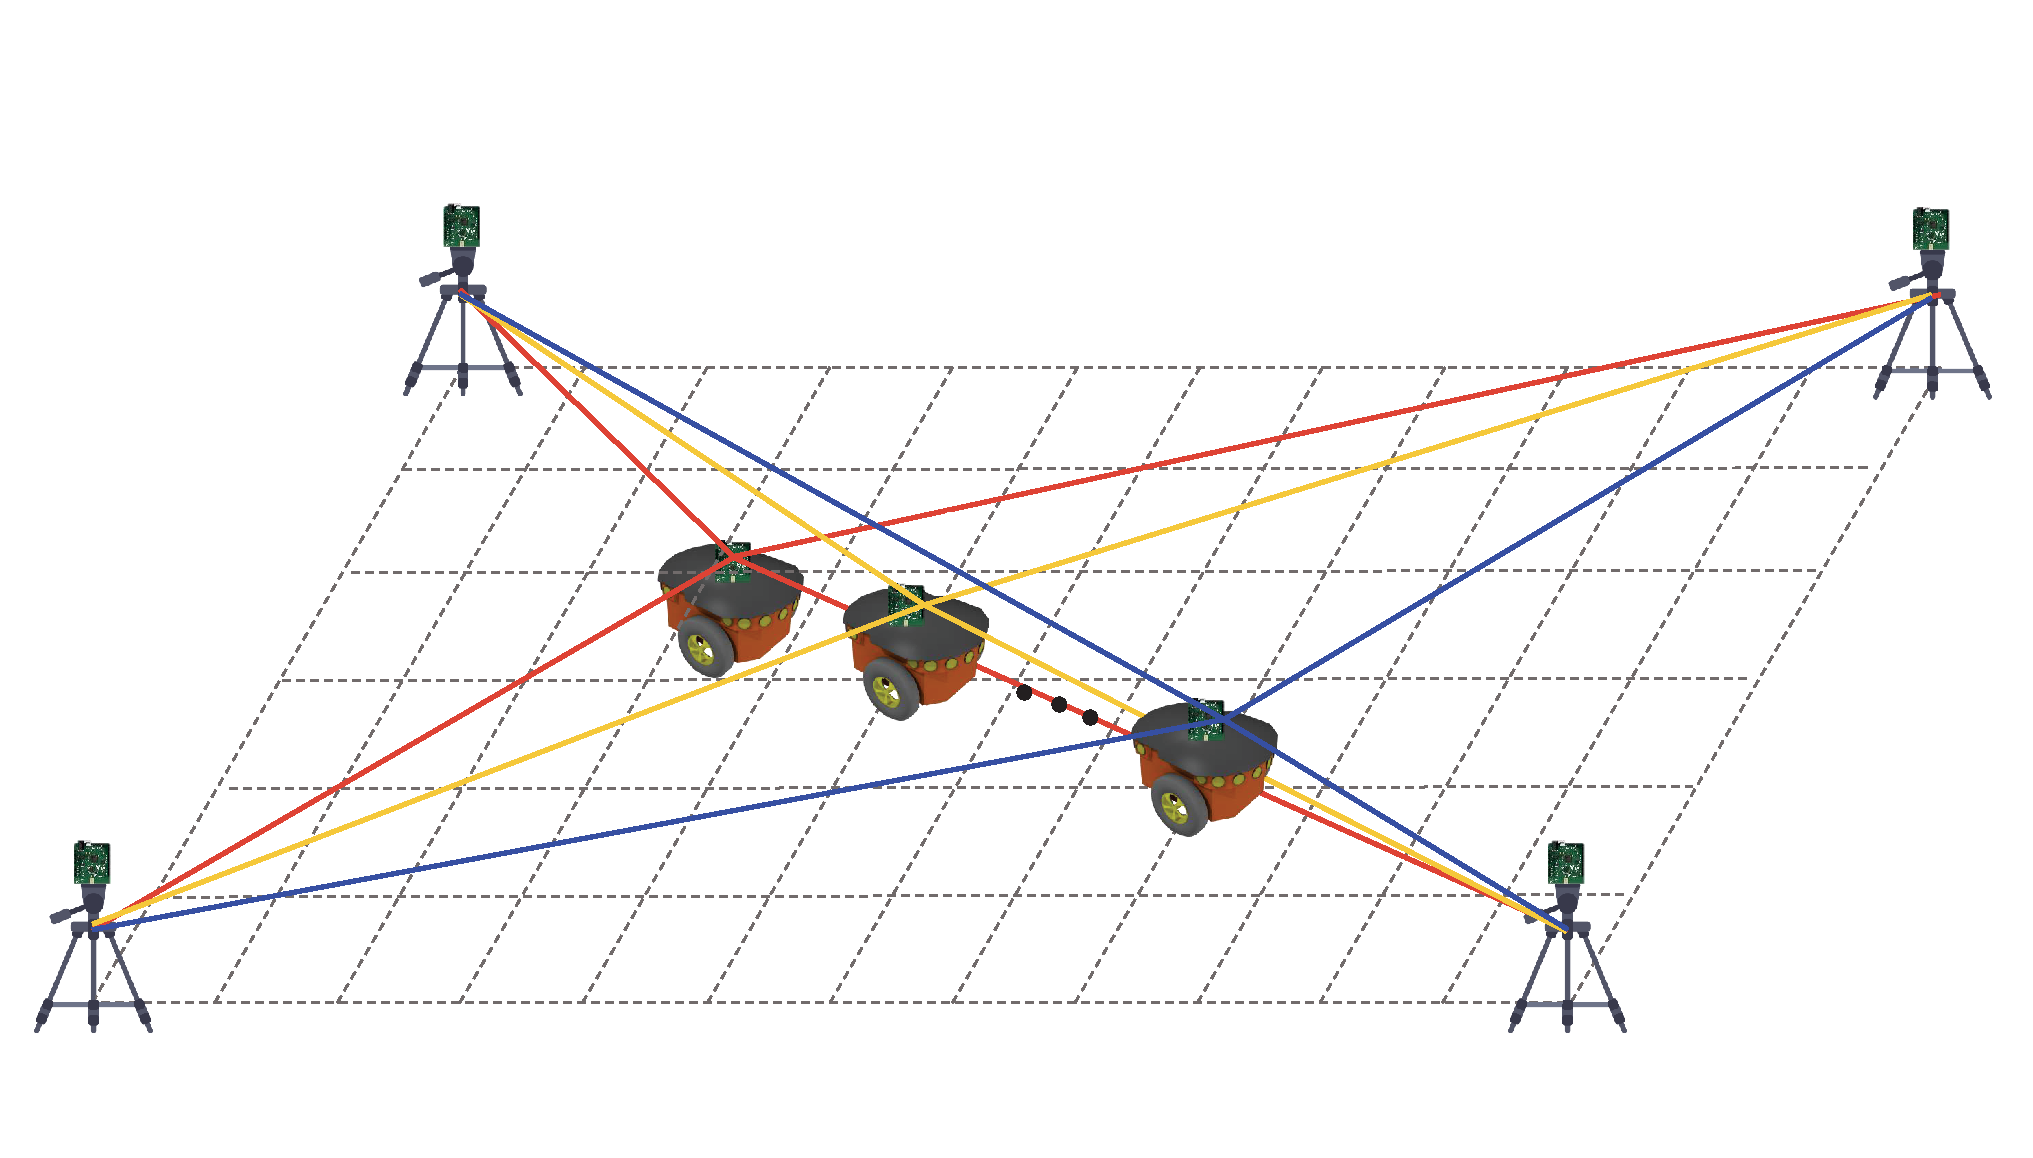
\includegraphics[height=4.5cm]{IROS2018_image_1}
	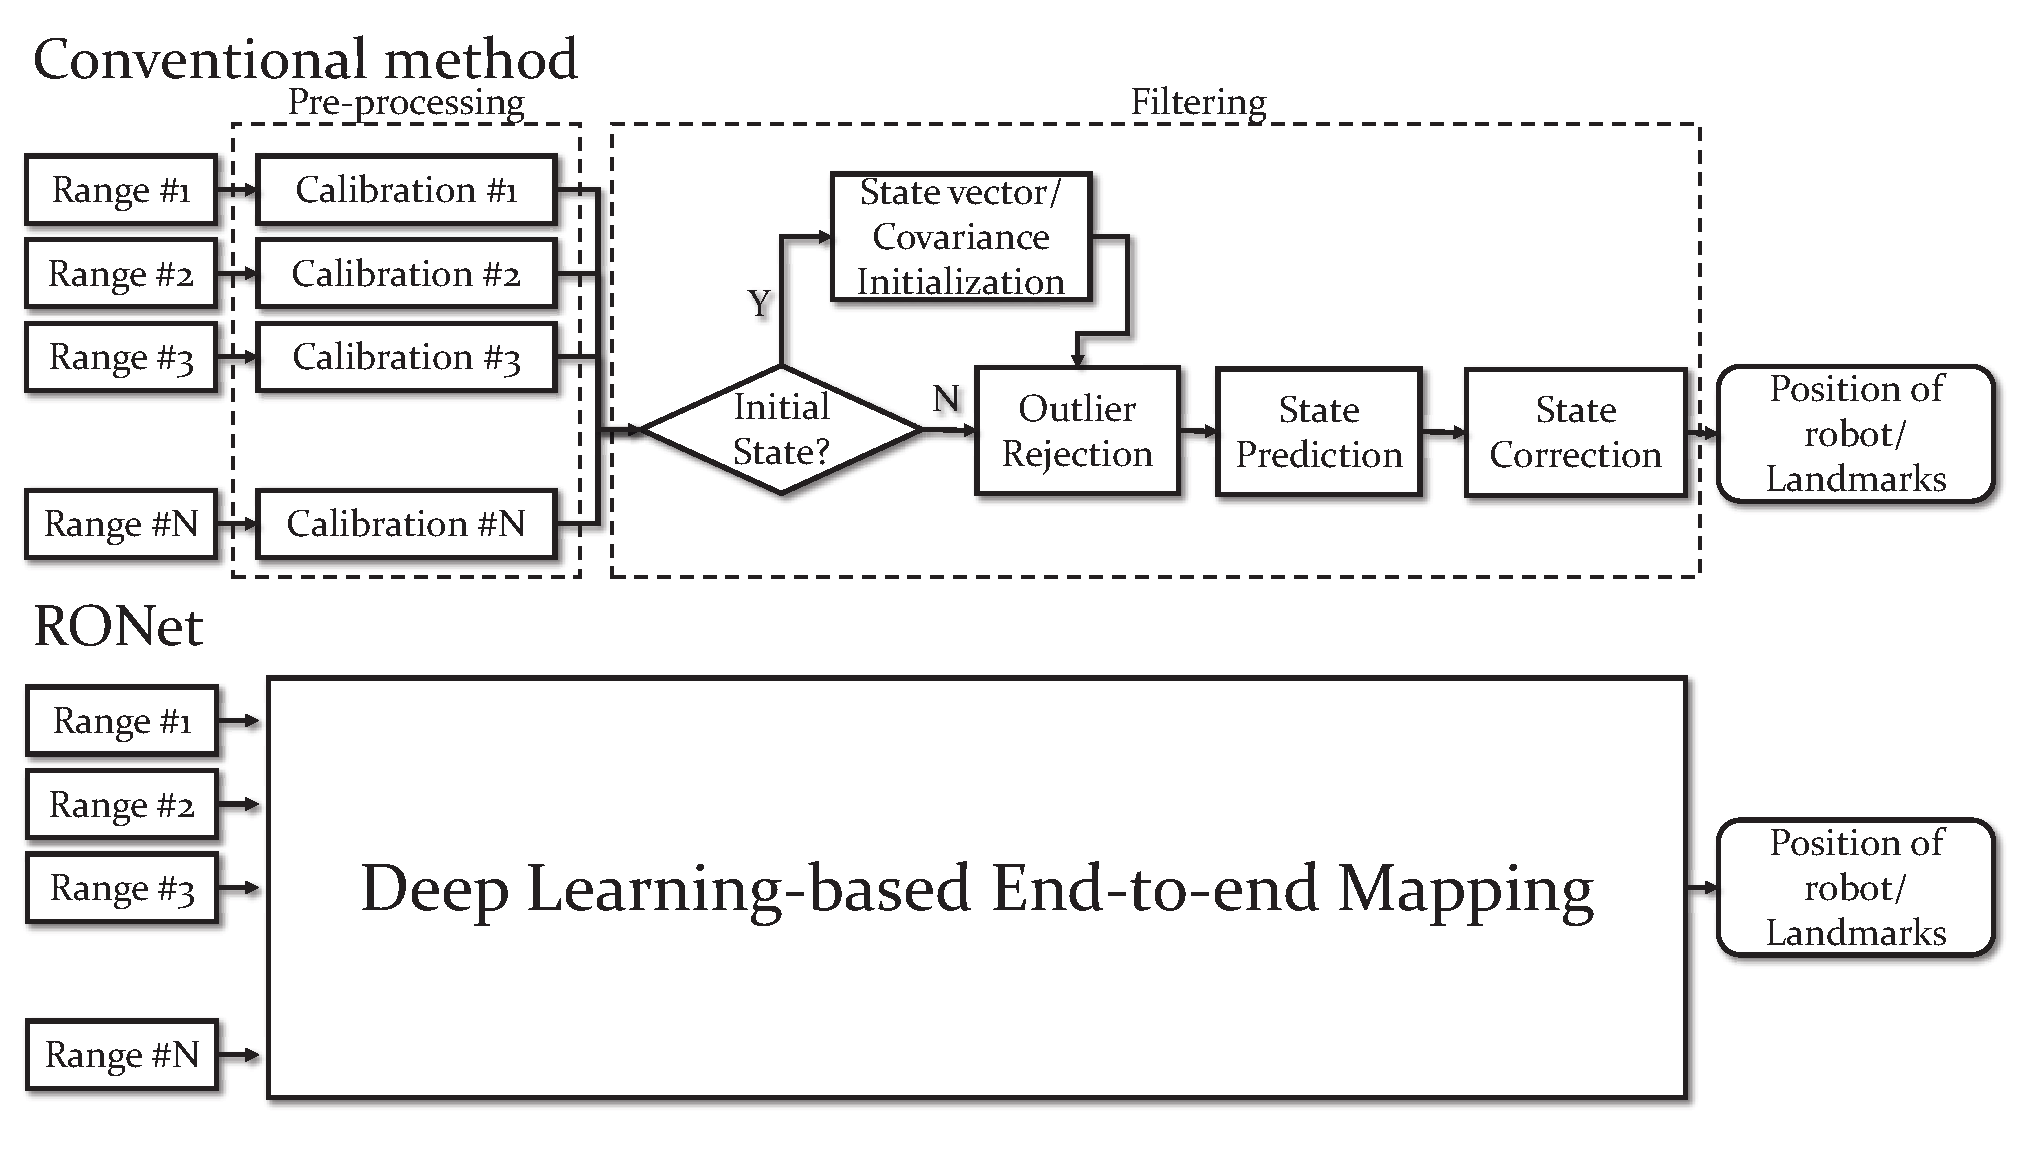
\includegraphics[height=5cm]{image/conventional_deep_comparsion}
	
	%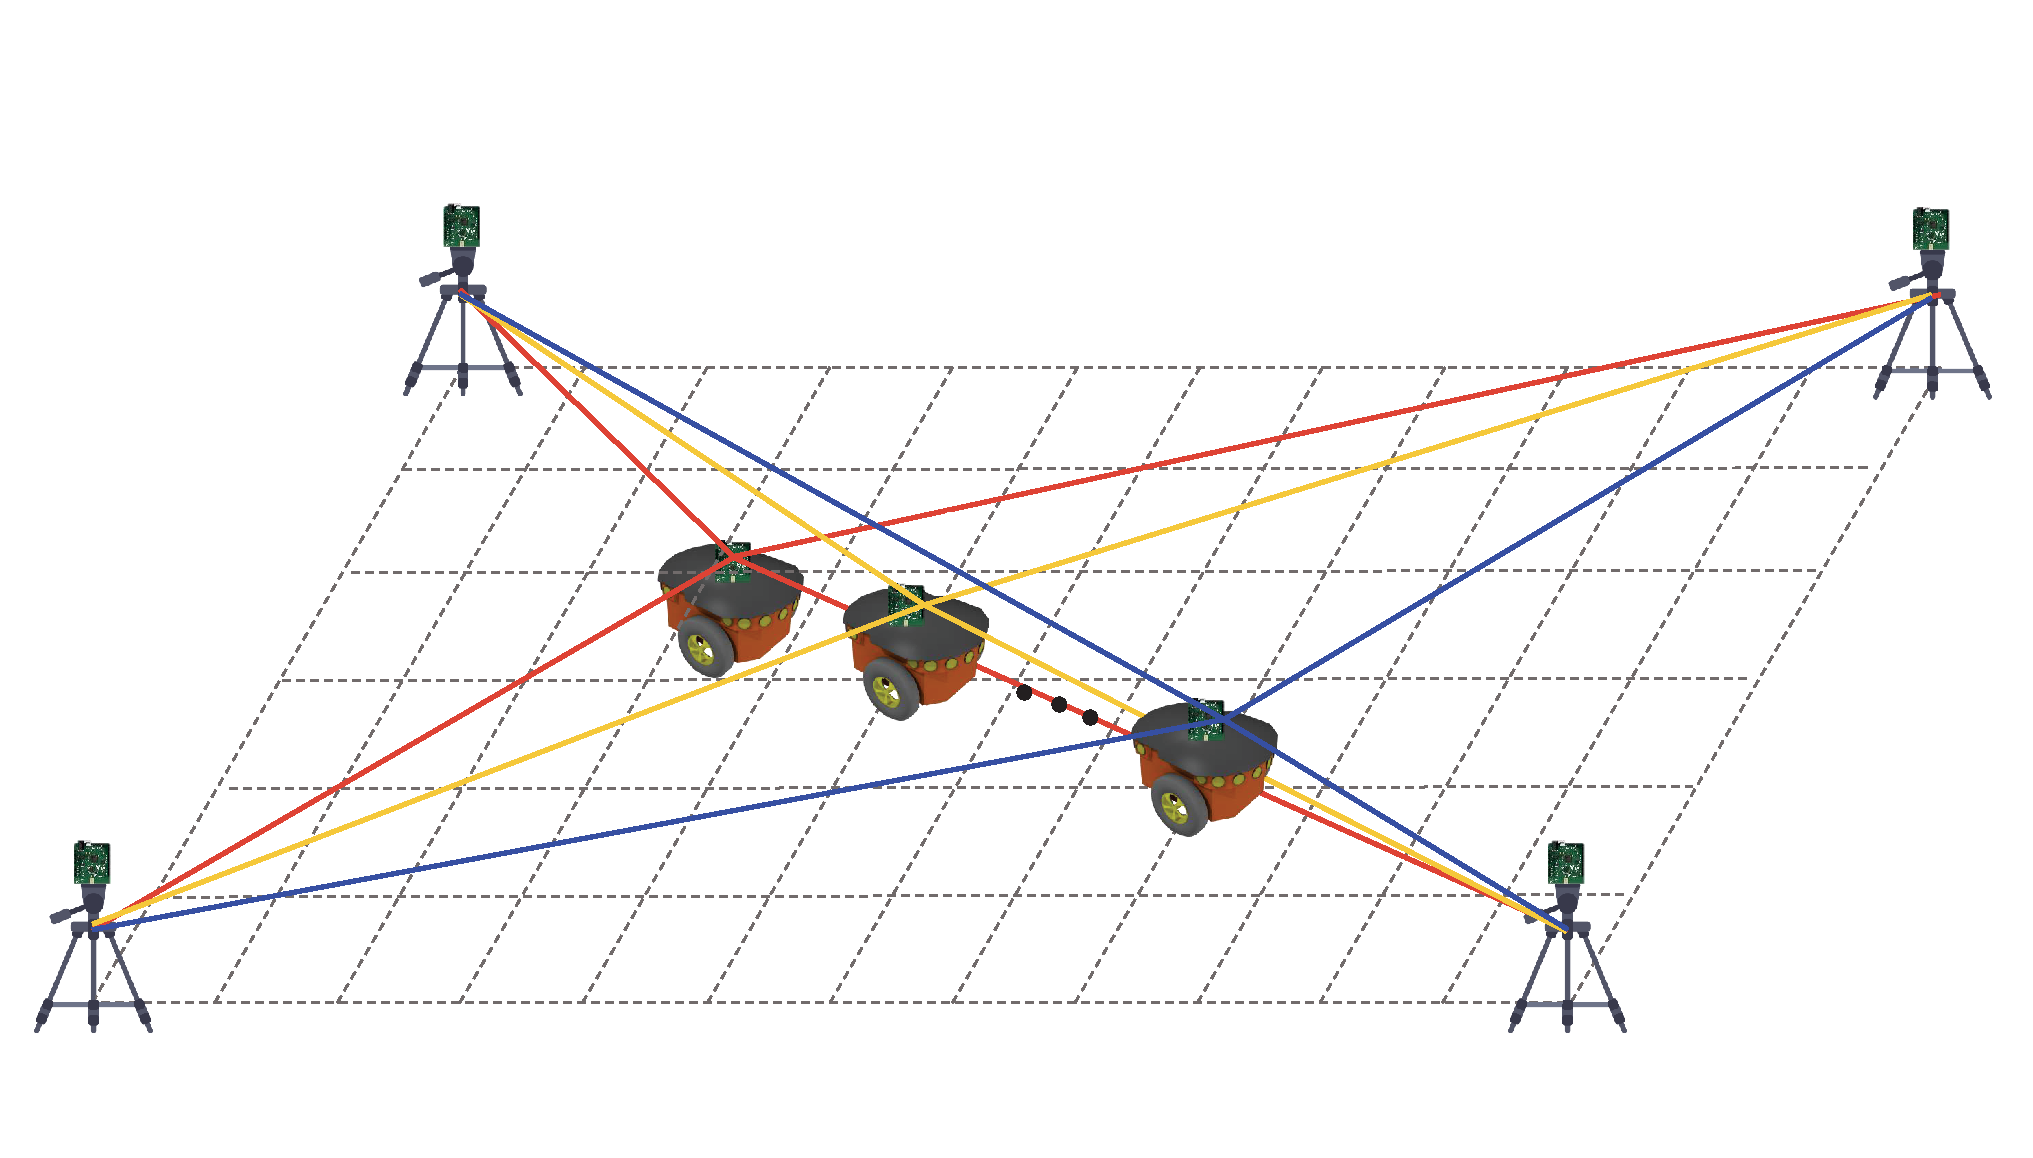
\includegraphics[trim={0 0 0 1cm}height=4.5cm]{IROS2018_image_1}
	\label{fig:example}
	%	}
	
	\caption{Comparison between a standard range-only localization or SLAM framework and our learning-based approach.}
	
\end{figure}

To alleviate these issues, many studies have been conducted based on probabilistic Bayesian inference framework and Monte-Carlo Bayesian filter, but in recent years, there have been attempts to solve these problems based on neural-network-based approaches\cite{rahman2009localization, abdelhadi2013efficient, kumar2016localization, lim2018effective}. With non-linear end-to-end mapping, the authors show feasibility. But most cases, they just utilized Multilayer Perceptron(MLP), which is beginning architecture of deep learning fields\cite{rahman2009localization, abdelhadi2013efficient, kumar2016localization}. In \cite{lim2018effective}, they exploit stacked bidireactional Long Short-Term Memory(Bi-LSTM) to cover noise of range observation by utilizing the chracteristics of it that takes temporal sequential value as input, yet they tested on the simulated environment. And all of them are not checked whether their learning-based approaches are real-time or not. 

In this paper, we propose a robust stacked BI-LSTM with residual attention, called RONet. To the best of our knowledge, it is a first approach to apply LSTM-based architecture to localize a mobile robot on the real-world in real-time using range-only measurement. Unlike conventional probabilistic-based algorithms, it does not need any preprocessing module, such as an calibration and outlier rejection.

Our contribution is threefold as follows:
\begin{itemize}
	%\setlength{\itemindent}{-.5in}
	\item We develop 3-stacked Bi-LSTM layers and attach residual attention layer for both improving performance and let the neural network be trained well so that our RONet shows the best performance when comparing the previous approaches.
	\item We also analyzed how the sequential length of the network affects performance and check robustness of our RONet with minimal number of anchors.
	\item We operate RONet on the Nvidia Jetson AGX Xavier and check the inference Hz is Real-time, about 32Hz. 
	
\end{itemize}

The rest of the paper is organized as follows: Section II overviews the related works. Section III describes our neural network in detail and defines the problem to be considered, and Section IV describes the experimental results. Finally, Section V summarizes our contributions and points to future work.

\section{Related Works}
\subsection{Conventional Range-Only Localization}

To localize a mobile robot using range measurements, there are two conventional approaches: Kalman Filter(KF)-based method and Particle Filter(PF)-based method. 

EKF \cite{olson2006robust}

 Besides, these measurements could have huge uncertainties caused by multipath fading channel(MPF) problem\cite{li2017novel} in real world. To alleviate these issues, many studies based on Kalman Filter(KF) algorithm or probabilistic approaches are conducted how to estimate state of the mobile robot and landmarks more precisely with covering the uncertainties. 

based on Ultra-Wide-Band(UWB), ultrasonic, laser-based beacon sensors. By virtue of this low-cost, small-size, acceptively accurate performance, and convenience of being installed, RO-SLAM 


h due to the convenience of trilateration that estimates the position of a receiver of range sensors if one only knows range measurement. For that reasons, range-only Simultaneous Localization and Mapping(RO-SLAM) methods are utilized popularly, which not only estimate the position of the receiver of range sensors, but also localize the position of range sensors regarded as features on a map, and studies have been conducted continuously in terms of probability-based approach\cite{blanco2008pure,blanco2008efficient,fabresse2013undelayed, shetty2018particle}. communicate with other wiresless sensors efficiently and conveniently. 


 \begin{figure*}[h]
	\centering
	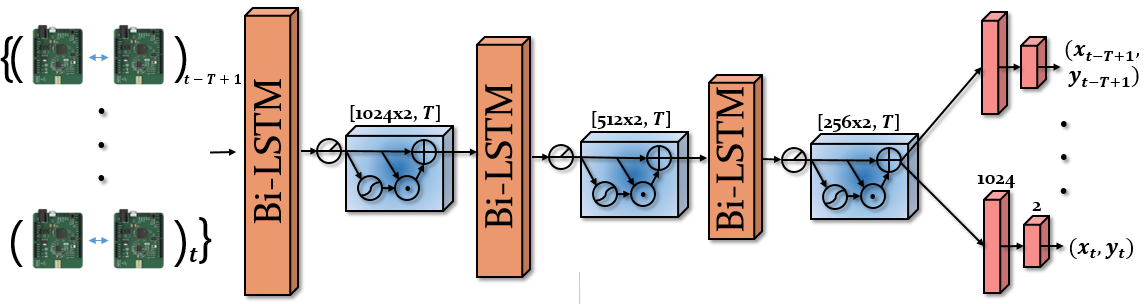
\includegraphics[width=0.9\linewidth]{image/network_figure}
	\caption{Our networks}
	\label{fig:our_network} 	
\end{figure*}

\subsection{LSTM-based Sequential Modeling}

As deep learning age has come\cite{lecun2015deep}, various kinds of deep neural architectures have been proposed for localization task related to robotics field\cite{kendall2016modelling, kendall2015posenet, gladh2016deep}. Especially, recurrent neural networks (RNNs), originated from Natural Language Process(NLP) area\cite{elman1990finding}, have been shown to achieve better performance in case of dealing with time variant information, thereby RNNs are widely utilized for sequential modeling such as not only speech recognition, but also pose estimation and localization.

And as Long Short-Term Memory (LSTM) architecture solves the \textit{long-term dependency}, which is the inherent issue to RNNs that become unable to learn the relationship of sequential informations as the time-sequential gap grows\cite{hochreiter1997long}, LSTM are actively introduced to learn longer-term contextual understandings. For example,in \cite{clark2017vinet}, the authors estimate the odometry by combination of RGB images and IMU sensor data and thy utilize the CNN unit for extraction of spatial information by images and LSTM unit for sequential modeling. in \cite{patel2018contextualnet, wang2017deepvo}, the architectures combined with CNN and LSTM are proposed for localization and odometry estimation tasks. LSTM unit extract sequential features from temporal outputs of CNN units. In \cite{walch2017image}, Walch \textit{et al.} propose the architecture that include CNN and LSTM units to regress camera pose for indoor and outdoor scenes. LSTM unit extract the sequential feature in an output of CNN unit. In addition, in \cite{song2017end}, the authors utilize multi-layered LSTM network for sequential action recognition by RGB-D images.


\subsection{Deep Learning for Range Only Localization}

Specifically, LSTM are also utilized to model low-dimentional sensor data by itself. In \cite{wang2018deepml}, they exploit LSTM for indoor localization with magnetic and light sensors. And in \cite{chen2018ionet}, they estimate 2D odometry via stacked bidirectional LSTM that takes only IMU sensor data as input. 

Our target, localization using range-only measurement, many authors employee neural networks-based approaches in Wireless Sensor Networks Fields(WSNs)\cite{rahman2009localization, abdelhadi2013efficient, kumar2016localization}, yet most networks are based on The Multilayer Perceptron(MLP). Their approach only map a set of range measurment on time $t$ to position so their approaches might have potential to unexpected sensor input. Other paper\cite{lim2018effective}, they utilize stacked bidirectional LSTM for localization a mobile robot takes sequential rnage measurements from anchors and the tag, but they only simulated on a ideal case, that MPF or unexpected noises not occur.

Therefore in this paper, we conduct experiments on a real-world to verify the feasibility to cover all noises of sensors with seqeuntial range data and compare these approaches.

!!!!!!!!!!!!!!!!!!!!!!

 An main advantage of neural networks-based approaches is that the neural networks enables themselves to recognize the position of the MNs quite accurately through the training even if there is no mathematical description. The neural networks also cover all noises that occurs when ANs and MNs interchange their signals. The authors show that their nerual networks-based approach have better performance than traditional approaches or machine learning-based approaches, yet most networks are based on The Multilayer Perceptron(MLP). In addition, the some authors just show the feasibility of their approaches, i.e., they trained and tested on the simulations situation. Plus, some authors let the neural networks infer the estimates on the two-dimensional space, but gap of the complexity of estimating position between on two-dimensional space and on three-dimensional using \textit{rank-deficient} measurements cannot be negligible.
 


\subsection{Residual Attention Layer}

A Attention layer is powerful module nowadays and mostly improves performance of neural network. Originally, neural networks treats information equally. But, using attention layer, neural networks can be ATTENDED what it should be examined closely. At the first time, attention is utilized at natural language processing area for improving translation performance\cite{luong2015effective}. But nowadays, attention layer is employed in many areas to improve the performance of the networks. For example, Jaderbeg \textit{et al.}\cite{jaderberg2015spatial} introduced the attention layer to let the neural networks attend to spatial information. In addition, attention is even utilized to pose estimation and optimization\cite{parisotto2018global}, detection\cite{zhu2018towards}, and video captioning\cite{xu2017learning} 

To precisely estimate the position of the tag node, it is important for the network to distinguish which is more meaningful context on time step \textit{T} to help contextual understanding of our  networks. So, we add the attention layer between the LSTM and the attention layer take on a role of a feature selector\cite{wang2017residual}. The equation of the attention machanism is as follows: 

 
\section{RONet}

In this chapter, we explain how our proposed residual attention-based stacked Bi-LSTM is implemented, as illustrated in Fig. \ref{fig:our_network}. 
In detail, we introduce the neural networks concepts that we choose for localizaing the tag node and then compare to those of other previous works. Finally, we describe how to set the loss function of our neural network 

\subsection{Long Short-Term Memory}

Unlike RNN that consist only of hidden state, in LSTM, cell state is added on the network. The cell state consists of the 3 gates to preserve the previous information and control the cell state: forget gate, input gate, and output gate and equations of those are as follows:


\begin{align}
f_{t} & =\sigma _{s}\big(W_{xf}\cdot x_{t}+W_{hf}\cdot h_{t-1}+b_{f}\big)\label{eq:forget}\\
i_{t} & =\sigma _{s}\big(W_{xi}\cdot x_{t}+W_{hi}\cdot h_{t-1}+b_{i}\big)\label{eq:input}\\
\tilde{c}_{t} & = \tanh\big(W_{xc}\cdot x_{t}+W_{hc}\cdot h_{t-1}+b_{c}\big)\label{eq:new_cell}\\
c_{t} & =f_{t}\odot c_{t-1}+i_{t}\odot\tilde{c}_{t}\label{eq:update}\\
o_{t} & =\sigma _{s}\big(W_{xo}\cdot x_{t}+W_{ho}\cdot h_{t-1}+b_{o}\big)\label{eq:output}\\
h_{t} & =o_{t}\odot \tanh\big(c_{t}\big)\label{eq:hidden}
\end{align}

where $\sigma _{s}$ is a kind of activation function, called \textit{sigmoid},  $f_{t}$, $i_{t}$, and $o_{t}$ respectively indicates the forget gate, input gate, and output gates, and $c_{t}$ denotes cell states. And $\odot$ denotes element-wise multiplication, called \textit{Hadamard product}. Entire gates are activated by sigmoid function and cell states are activated by $\tanh$ function.

The Forget gate layer, $f_{t}$, decides how much information to forget based on previous hidden state, $h_{t-1}$, and present input, $x_{t}$. Next, the input gate, $i_{t}$, decides how much information to embrace when updating the cell state. After that, $c_{t}$ is updated by the cell state layer based on $f_{t}$, $i_{t}$, and candidate cell state, $\tilde{c}_{t}$ \eqref{eq:update}. In addition, output gate layer, $o_{t}$, sereves as a filter, which means $o_{t}$ determine what values are going to output \eqref{eq:output} in such a way as that $h_{t}$, is updated based on $o_{t}$ updated cell state, $c_{t}$ \eqref{eq:hidden}. 

\subsection{Stacked Bidirectional LSTM}

\begin{figure}[h!]
	\centering
	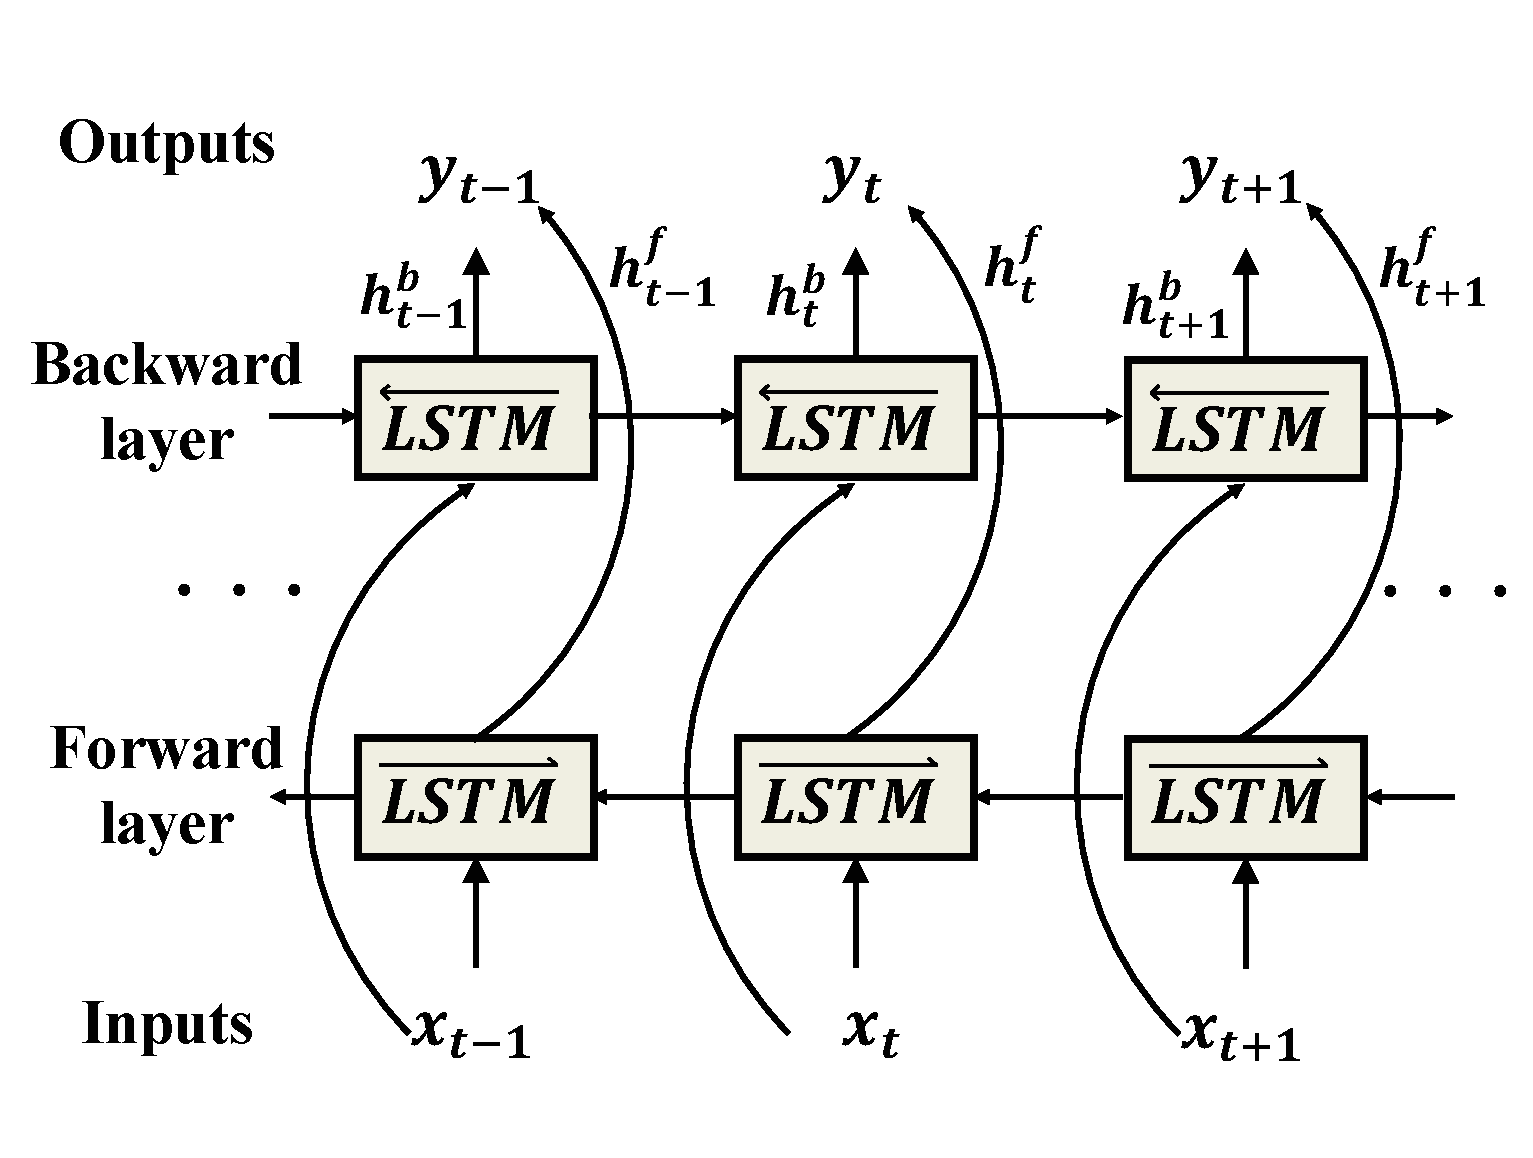
\includegraphics[width=.9\linewidth]{image/bidirectional_LSTM_revised}
	\caption{Architecture of the Bidirectional LSTM(Bi-LSTM). bidirectional LSTM consist of 2 LSTMs:  one forward LSTM layer}
	
	%$\overrightarrow{LSTM}$, and one backward LSTM layer, $\overleftarrow{LSTM}$}
	\label{fig:bidirectional_revised}	
\end{figure}

Like the fact that the deeper the architecture of neural networks, the better their performance\cite{simonyan2014very, he2016deep}, many authors have analyzed variations of LSTM architecture and find out that stacking multiple layers of the LSTM improve the performance for many tasks\cite{graves2013hybrid, graves2013speech,ullah2018action}. Besides, Bidirectional RNNs are introduced\cite{schuster1997bidirectional} to extract well-described context. It has one forward LSTM, $\overrightarrow{LSTM}$, and one backward LSTM, $\overleftarrow{LSTM}$, running in reverse time so that the network exploits not only previous forward context to up update $h_{t}$ and $c_{t}$ but also future backward context as well, as FIGURE. \ref{fig:bidirectional_revised} shown. 

For these reasons, we adopt stacked bidirectional LSTM architecture to model the system. By virtue of these increased non-lineary caused by a number of stacked layers, the network could model more complex localization taking UWB-rangings as input including unexpected noise and MPF problems. And, we judge that Bi-LSTM would be more helpful to produce more appropriate context considering both past and future at the same time

Therefore, we construct our networks by stacking three LSTM to increase the non-linearity. Note that stacking over than three LSTM doesn't show the improvement of performance. We deem that this problem could comes from the sigmoid function and $tanh$ function that compose the part of LSTM. These activation functions cause the \textit{vanishing gradient problem}\cite{pascanu2013difficulty}, which the networks fail to training due to the fact that the gradient is getting closer to zero during the backpropagation. Consequently, we put the ReLu function between LSTMs to avoid the vanishing gradient problem\cite{nair2010rectified}, instead of stacking more LSTM to increas non-linearity. And experiments shows that reducing the hidden size of next LSTM layer when the features are fed into the LSTM layer slightly increases preformance, but reducing dramatically rather cause underfitting. In conclusion we decide to set the size of the layers as 1024-512-128. Note that we adopt Bi-LSTM, acutual feature size is 2048-1024-256. And end part of the LSTMs, fully connected layers are attached to predict the mobile robot's position based on the sequential features processed by the LSTMs.  

\subsection{Residual Attention layer}

A Attention layer is powerful module nowadays and mostly improves performance of neural network. Originally, neural networks treats information equally. But, using attention layer, neural networks can be ATTENDED what it should be examined closely. In other words, attention layer take on a role of a feature selector\cite{wang2017residual}. To precisely estimate the position of the tag node, it is important for the network to distinguish which is more meaningful context on time step \textit{T} to help contextual understanding of our networks. The equation of original attention machanism is as follows:  

\begin{equation}
H(x)=M(x)\odot x
\end{equation} 

where $x$ denotes the output of previous neural network layer, $H(x)$ denotes the output of the attention layer to be passed to the next neural network layer and $M(x)$ denotes the attention mask. By element-wise multiplying $x$ by $M(x)$, attention layer makes the network weight more crutial information. 

Despite of the improvement of the performance, the attention layer has potential risks that it may dilutes the features because attention mask ranges over 0 to 1. So we adopt residual attention layer to alleviate this problem as follows\cite{wang2017residual}:

\begin{equation}
H(x)=\left(1+M(x)\right)\odot x
\end{equation} 

As blue cuboid shape in the FIGURE \ref{fig:our_network} shown, this idea is originated from the Residual Net(ResNet)\cite{he2016deep} that has skip connection in such a way as to mitigate aforementioned dilution problem and help the network to be trained well. Likewise the ResNet, residual attention also has other branch to calculate how much to attend and the branch is joined with original feature vector $x$. Each hidden state has each residual attention layer so that these attention modules can determine which time stamp has more fruitful meaning and deliver the output to next bidirectional LSTM.

\subsection{Training loss}

In this section, we describe the method for training our network. Generally, let $n$ be the number of anchor nodes, data set, $L_{t}$, measured by each anchor node and tag node and ground truth of 2D position, $Y_t$, are represented on the time step $t$ as follows:

\begin{equation}
L_{t} = (l_{1}, l_{2}, ..., l_{n})_{t}
\end{equation}
\begin{equation}
Y_t = (x_t, y_t)
\end{equation}

where $l_{i}$ denotes the the distance between $i^{th}$ anchor node and the tag node. Note that our neural network does not only take a set at the time $t$ but takes sets based on the sequential length of input to our network, $T$ as follows:

\begin{equation}
%$L = \left\{(X_t, Y_t)\right \}$ 
\mathbb{L}_t = \left\{L_{t-T+1}, L_{t-T+2}, ..., L_t\right\} 
\end{equation}
\begin{equation}
\mathbb{Y}_t = \left\{Y_{t-T+1}, Y_{t-T+2}, ..., Y_t\right\}
\end{equation}

Conseqeuntly, neural network could be optimized to be able to localize the mobile node by being trained using the train data set $\mathbb{D}$ as follows:  

\begin{equation}
%$L = \left\{(X_t, Y_t)\right \}$ 
\mathbb{D} = \left\{(\mathbb{L}_{T-1}, \mathbb{Y}_{T-1}),...,(\mathbb{L}_t, \mathbb{Y}_t),...\right\} 
\end{equation}

Therefore, Let $\Theta$ be the parameters of our network model and our final goal is to find optimal parameters $\Theta^{*}$ for precise localization by minimizing $L_2$ loss term. The $L_2$ loss term indicates mean square error(MSE) of Euclidean distance between the normalized ground truth position $\mathfrak{N}(Y_k)$ and estimated position $\hat{Y_k}$ as follows:

\begin{equation}
\Theta^{*} = \underset{\Theta}{\mathrm{argmin}} \frac{1}{N}\frac{1}{T} \sum_{k=T-1}^N\sum_{m=k-T+1}^k \parallel \mathfrak{N}(Y_m) - \hat{Y_m} \parallel^{2}
\end{equation}  

\begin{figure*}[h]
	\centering
	\begin{subfigure}[b]{0.3\textwidth}
		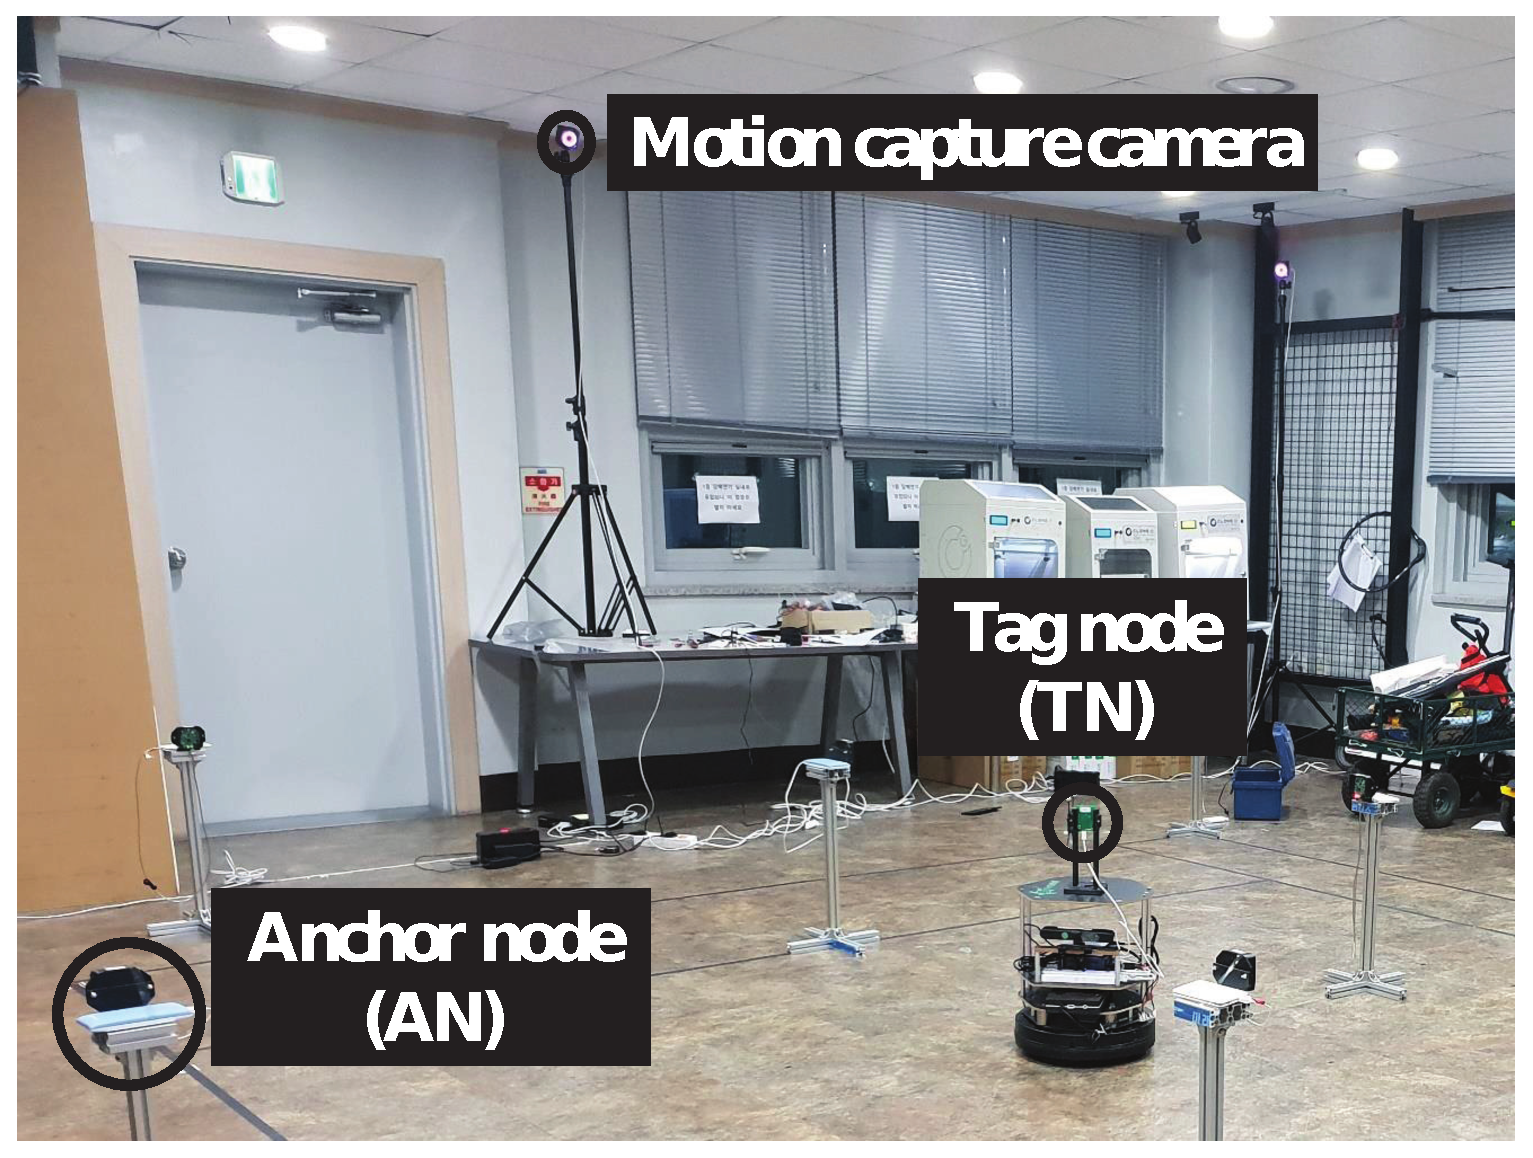
\includegraphics[width=\textwidth]{image/system_whole_picture}
		\caption{A gull}
		\label{fig:whole_system}
	\end{subfigure}
	%add desired spacing between images, e. g. ~, \quad, \qquad, \hfill etc. 
	%(or a blank line to force the subfigure onto a new line)
	\begin{subfigure}[b]{0.3\textwidth}
		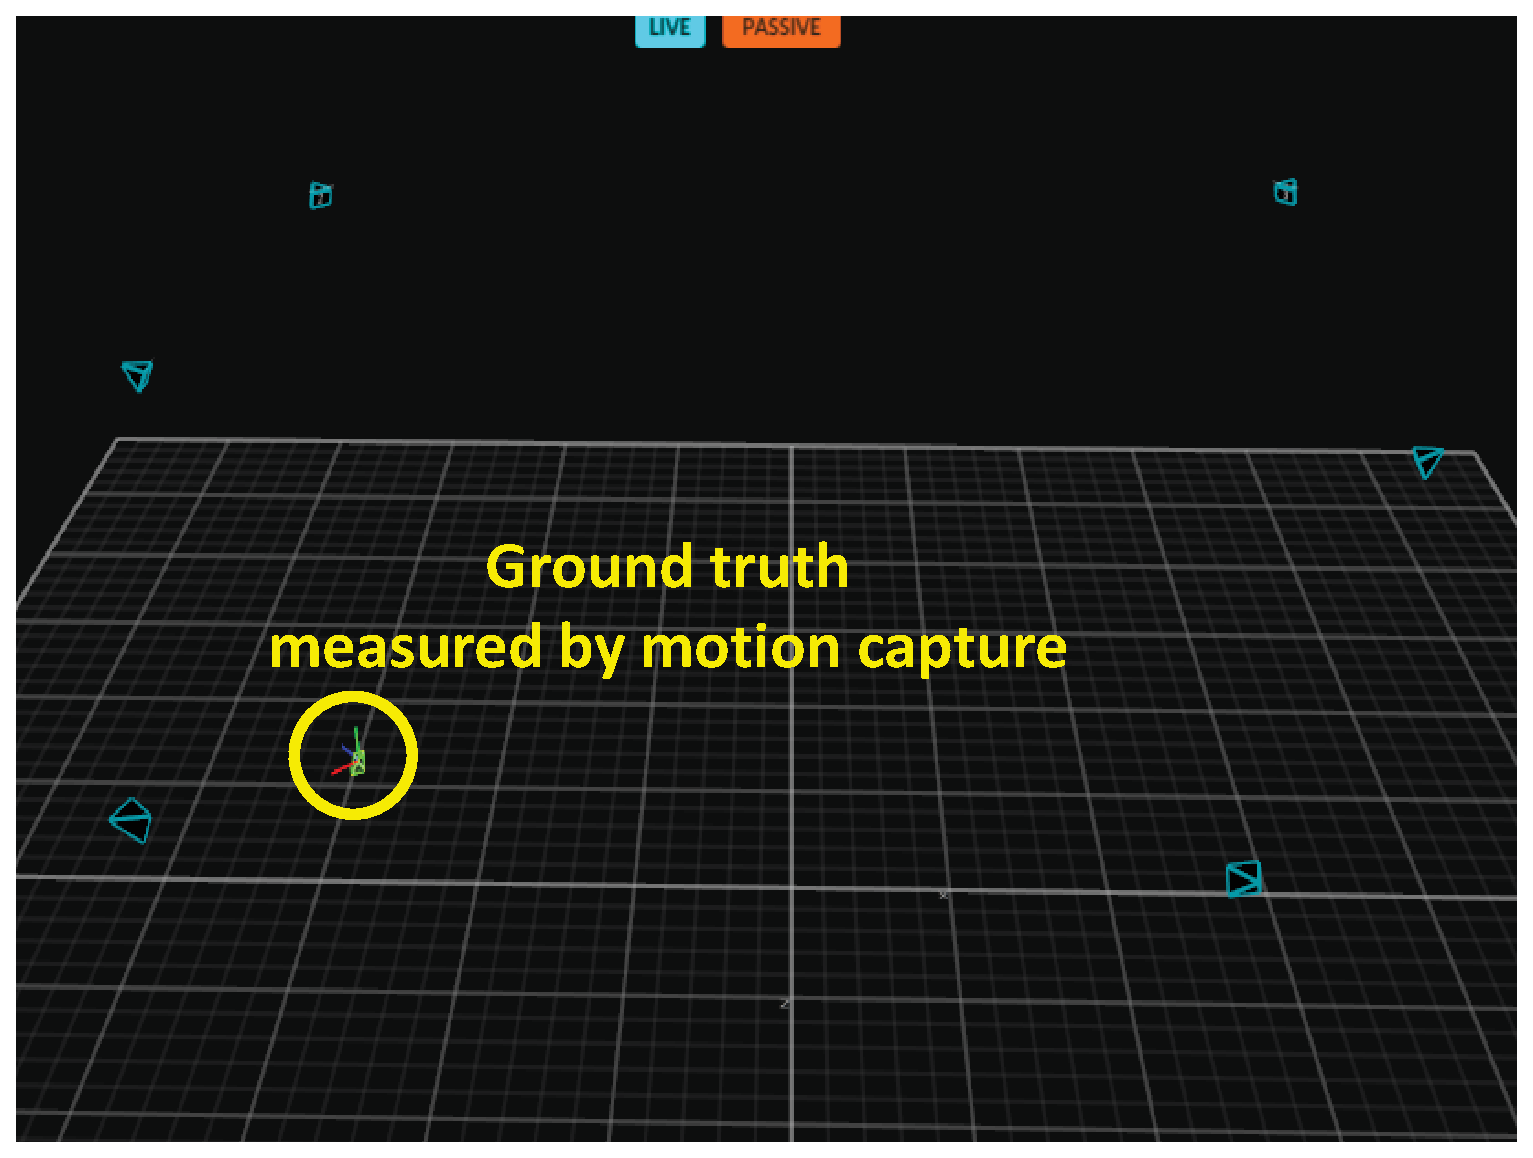
\includegraphics[width=\textwidth]{image/system_mocap}
		\caption{A tiger}
		\label{fig:Optitrack_figure}
	\end{subfigure}
	%add desired spacing between images, e. g. ~, \quad, \qquad, \hfill etc. 
	%(or a blank line to force the subfigure onto a new line)
	\begin{subfigure}[b]{0.3\textwidth}
		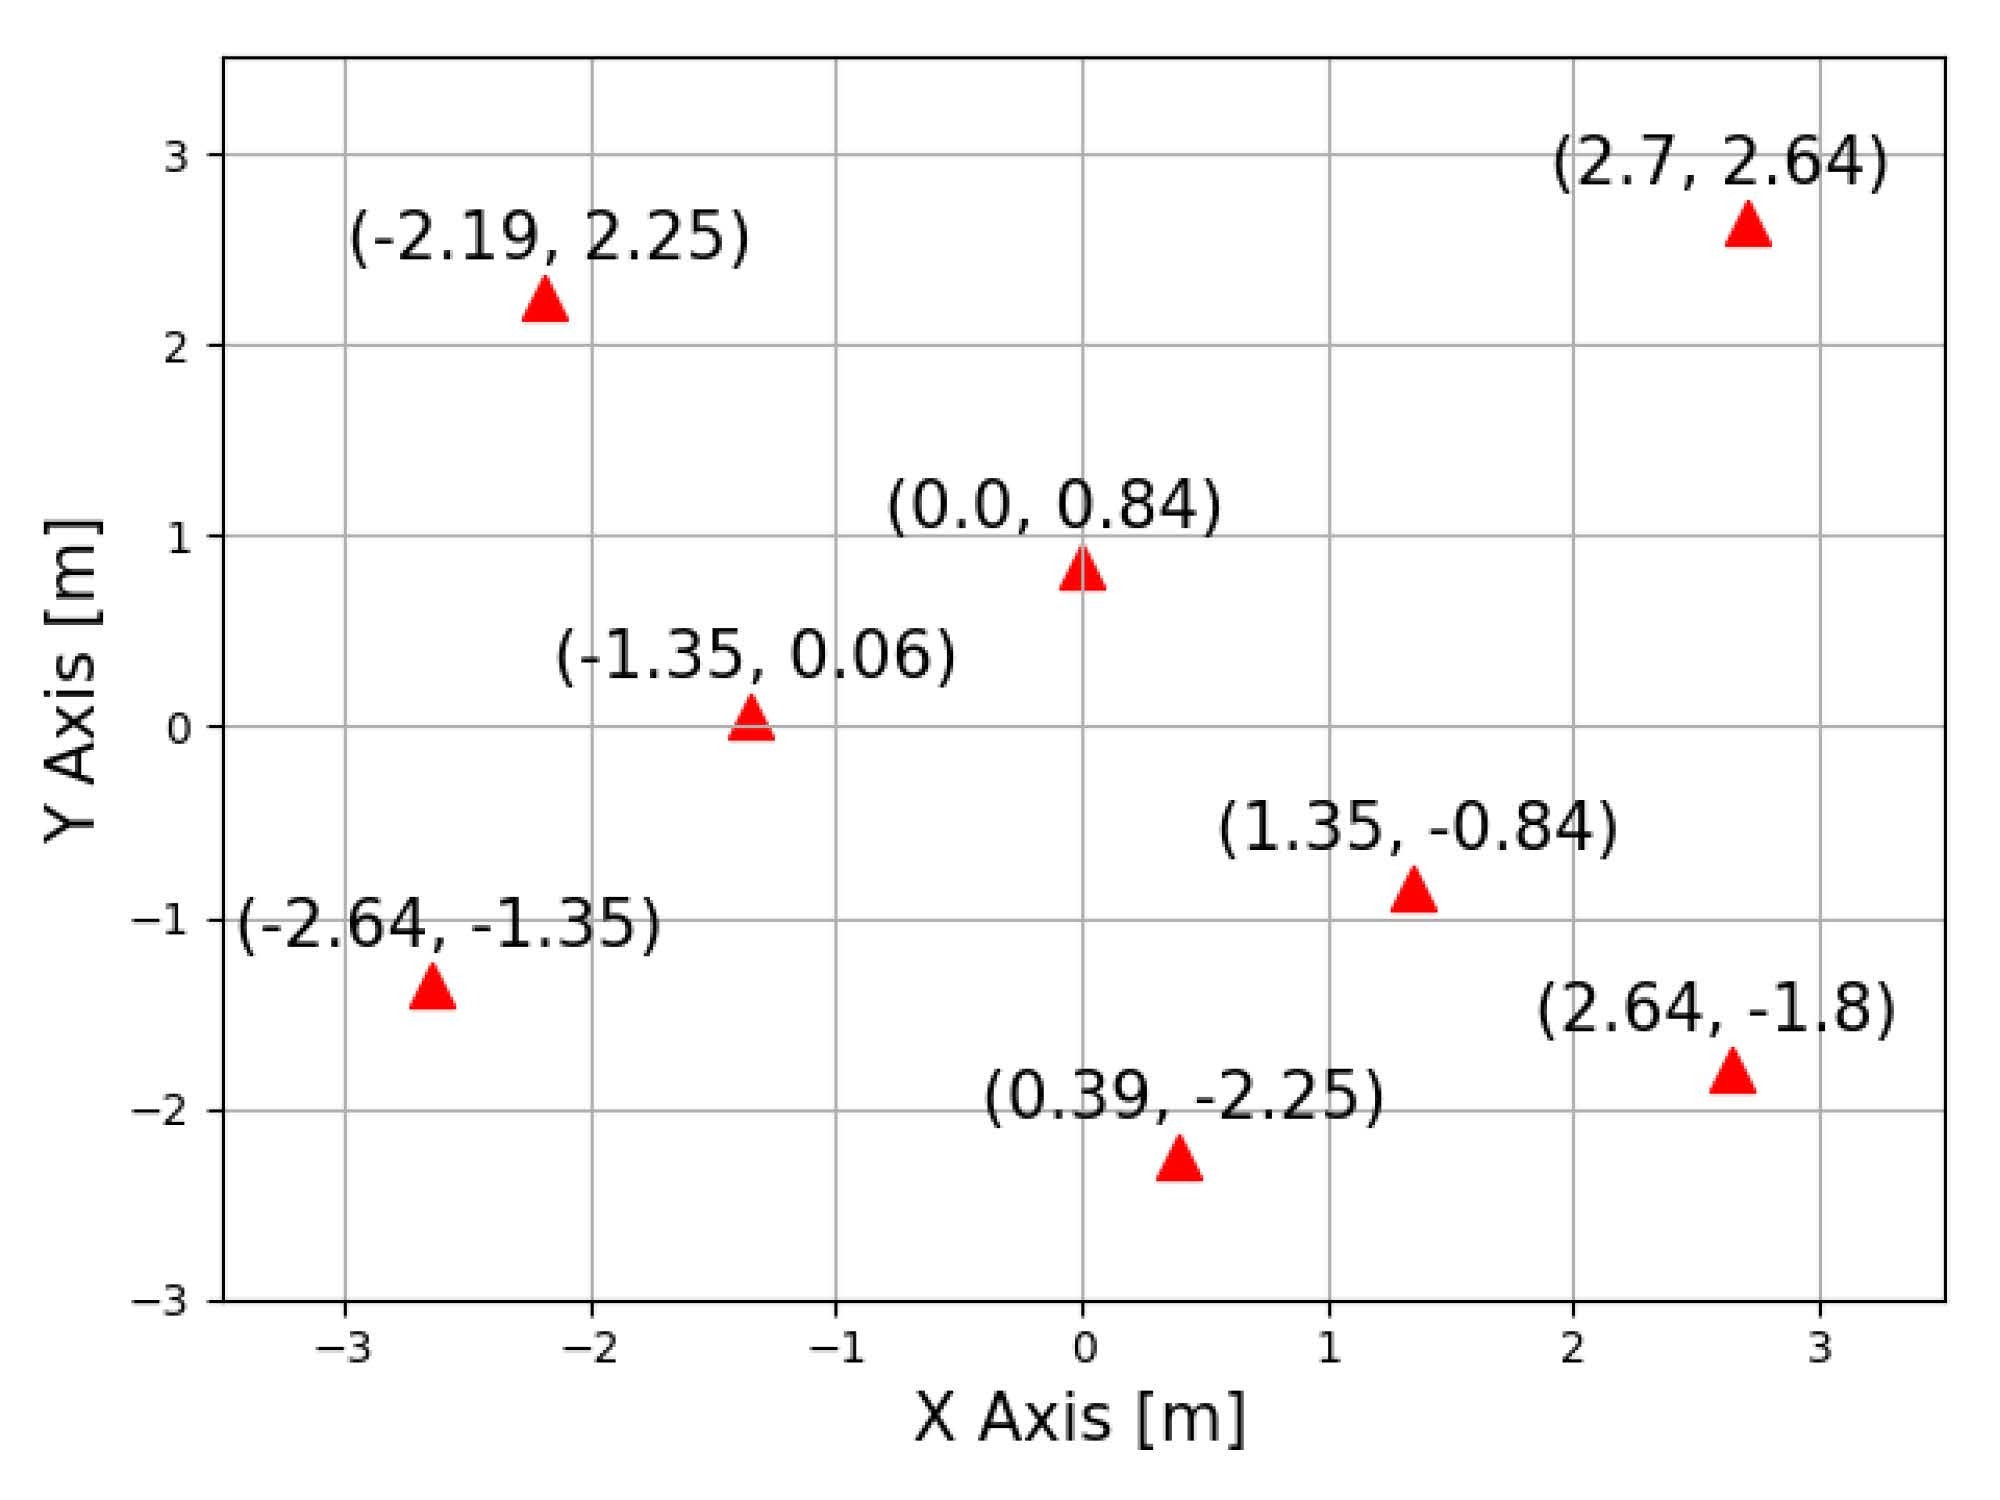
\includegraphics[width=\textwidth]{image/system_exact_position}
		\caption{A mouse}
		\label{fig:Exact_position}
	\end{subfigure}
	\caption{Pictures of animals}\label{fig:animals22}
\end{figure*}

\section{Experimental Results}
\subsection{Experimental environment}

Our experimental system consists of a UWB sensor tag node attached on the mobile robot platform  and eight anchor nodes that take roles of a UWB transceiver, 6 Optitrack Prime 13 motion capture cameras, a Nvidia Jetson AGX Xavier, which is a SFF(small-form-factor) computer that has a GPU. Fig. \ref{fig:whole_system} shows our experimental environment briefly and how to the anchor nodes and the tag node are attatched. And we use the mobile platform, called iClebo Kobuki from Yujinrobot.

The tag node receives the signal and measures the range between two devices based on time of flight(TOF) and Received Signal Strengh Indication(RSSI). Each UWB transceiver, DW1000 UWB-chip made by Decawave, supports 6 RF bands from 3.5 GHz to 6.5 GHz. It measures in cm-level accuracy.

 Deep learning framework used for our network is tensorflow-gpu 1.7.0 on python 3.5.2
 
\subsection{Acquisition of the Train/Test data}
UWB sensor anchors are installed randomly in the region where motion capture camaras are acceptable, as Fig. \ref{fig:Exact_position} shown. These anchor nodes transmit the UWB signal to tag node that is attached to the mobile robot and the Optitrack motion capture cameras also transmit the ground truth data to the SSF computer by utilizing Robot Operating System(ROS).

Note that these two dat are transmitted by different frequency: range measurements are gathered with a frequency of almost 27Hz, yet the ground truth data are 120Hz. So we synchronize these two data based on the range measurements' Hz. More specifically, we set an independent thread so that this thread select the ground truth data of the nearest time based on the UWB-range measurements, concatenates and saves these data at the same time.

And the mobile robot moves in this sapce by manually. All the trajectories are different. After collecting whole datasets, we separate the entire dataset to three types: one are the training datasets, another are for the validation datasets, and the other is for test dataset. On the test dataset, only range measurements are taken as input to the network.

\subsection{Training the Network}

To train our network, the Adam optimizr is exploited to train the
network during 1000 epochs with 0.0002 learning rate, 0.7
decay rate, and 5 decay step. Besides, Dropout is introduced
to prevent the models from overfitting.

\subsection{Localization Results}

Pass


To improve the performance of our proposed networks, we check which seqeunce length is optimal for localization of MN. And then, we implemented and trained other previous networks to compare their performance when our real-world data are given as input. We set three test trajectory cases: a square path, a verical and horizontal winding path, and a diagonal winding path. 

\subsubsection{Performance according to the sequence length}

Even though LSTM solve the long term dependency problem, we thought that it would not always make neural network perform better as sequence length become more longer. So, as part of turning hyperparameters, we modified sequence length of our network in a variety of numbers to find optimal sequence length.   

As illustrated in FIGURE. \ref{fig:paths}, The train data are gathered by the robot that arbitrary moves on the region where the motion capture camera cover. The neural network takes distances measured by each AN and a MN as input and outputs robot's position. The Root-Mean-Squared Error (RMSE) results of trajectory prediction with respect to sequence length are shown in FIGURE. \ref{fig:seq_length} and specific figures are shown in Table \ref{table:RMSE_sequence}.

As a result, we found that there is a trade-off between robustness and improvement of general performance according to the sequence length. Figure. \ref{fig:seq_length} show that as longer the sequence length, as more inaccurate the mean performance. This is because it is hard for the neural architecture to train the chracteristics of the sequential data. In other words, as sequence length become longer, the tendency of the values may be different due to accumulation of different patterns of system noises even if the data is acquired by moving to a similar path in the train data. Note that network with longer sequence length tend to have less error variance and more a ability to generalize the situation since they could utilize more extended temporal information. By doing so, the nerual network have the ability to suppress the disturbance caused by noises.

%Similarily, as sequence length become shorter, it is less difficult for the neural architecture to understand the chracteristics of the sequential data by virtue of the less accumulation of different patterns of system noises. Note that in most cases, the network constructed by the shorter sequential length tend to estimate the position more precisely than those with longer sequential lengths. However, 생t becomes a double-edged sword because temporal information is also reduced accordingly in such a way as to week to the noises, having larger error variance.



%sequence length가 길어질수록 netowrk가 그 sequential data를 일반화 시키는 게 어렵다
%In other workds, sequence length만큼 끊어서 input으로 받기 때문에 sequential한 경향성에 대해 적절한 output을 내게 학습을 하는데, sequence가 길어지게 되면 길어지는 만큼 그 상황이 특수해져서 비슷한 특성을 지닌 input이 줄기 때문이다????
%길이가 길어짐에 따라 noise에 대한 방해를 더 길어진 temporal information을 활용해서 억누를 수 있다.
%On the other hand, 짧아질수록 좋지만 경향성을 학습?

\begin{figure}[h!]
	\centering
	
\includegraphics[width=0.9\linewidth]{image/be_updated}
	\caption{Error bar graph of RMSE with respect to sequence length}
	\label{fig:seq_length} 	
\end{figure}
\begin{table}[]
	\centering
	\begin{tabular}{ccccc}
		\hline
		\multicolumn{5}{c}{The results of RMSE {[}cm{]}}   \\ \hline
		\# of anchors & EKF RO-SLAM & MLP & Bi-LSTM & Ours \\ \cline{2-5} 
		3             & 1           & 2   & 3       & 4    \\
		5             & a           & b   & c       & d    \\
		8             & A           & B   & C       & D    \\ \hline
	\end{tabular}
\end{table}

\begin{table}[h]
	\centering
	\caption{Root mean squared error of each case}
	\begin{tabular}{clllll}
		\toprule
		\multicolumn{6}{c}{The results of RMSE[cm]}                         \\
		\midrule
		& \multicolumn{5}{c}{Sequence length} \\  \cmidrule{2-6}
		
		\multicolumn{1}{l}{} & 2     & 3       & 5      & 7    & 10  \\
		Test1                & 2.84  & 2.88    & \textbf{2.78}   & 3.65 & 4.16 \\
		Test2                & 3.61  & 3.63    & \textbf{3.57}   & 3.84 & 4.18 \\
		Test3                & \textbf{2.93}  & 3.21    & 3.03   & 3.62 & 3.93 \\
		\bottomrule 
		
	\end{tabular}
	\label{table:RMSE_sequence}
\end{table}

\subsection{Performance comparison Result}

The results of trajectory prediction are shown in Fig. 3(a) and Fig. 3(d) and
Root-Mean-Squared Error (RMSE) are shown in Table 1. Performance is better
in order of stacked Bi-LSTM, Bi-LSTM, LSTM and GRU. In case of GRU, it
has only two gates which is less complex structure than LSTM [27]. However,
due to GRU's less complexity, GRU has less number of neurons than LSTM so
their non-linear mapping achieves less performance. Likewise, Bi-LSTM consists
of two LSTMs to process sequence in two directions so that infer output using
the correlation of the backward information and the forward information of the
sequences of each time step with its two separate hidden layers. Thus, Bi-LSTM
has better nonlinear mapping capability than LSTM. For similar reasons, stacked
Bi-LSTM is the architecture that stacks two Bi-LSTMs, so inference performance
is better than Bi-LSTM. As a result, the stacked Bi-LSTM showed the best
performance among unit RNN architectures. Therefore, we can conclude that
the performance improves as the non-linearity of the architecture increases.


\begin{figure*}[h]
	\centering
	\begin{subfigure}[b]{0.3\textwidth}
		
\includegraphics[width=\textwidth]{image/be_updated}
		\caption{A gull}
		\label{fig:gull2342}
	\end{subfigure}
	%add desired spacing between images, e. g. ~, \quad, \qquad, \hfill etc. 
	%(or a blank line to force the subfigure onto a new line)
	\begin{subfigure}[b]{0.3\textwidth}
		
\includegraphics[width=\textwidth]{image/be_updated}
		\caption{A tiger}
		\label{fig:tige234r2}
	\end{subfigure}
	%add desired spacing between images, e. g. ~, \quad, \qquad, \hfill etc. 
	%(or a blank line to force the subfigure onto a new line)
	\begin{subfigure}[b]{0.3\textwidth}
		
\includegraphics[width=\textwidth]{image/be_updated}
		\caption{A mouse}
		\label{fig:mous234e2}
	\end{subfigure}
	\caption{Pictures of animals}\label{fig:a234nimals22}
\end{figure*}

!!!!!!!!!!!!!!!!!
We also verified effectiveness of attention layer. It was confirmed that the performance of the networks with the attention layer is improved compared to the networks without the attention layer.
We also provide statistical analysis from simulations demonstrating that
our new approach can cope with highly noisy sensors and
reduces in one order of magnitude the average errors of the
method proposed
!!!!!!!!!!!!!!!!!


\section{Conclusion}

In this paper, we proposed a novel approach to range-only SLAM using multimodal-based RNN models and tested our architectures in two test data.

Using deep learning, our structure directly learns the end-to-end mapping between distance data and robot position. The multimodal bidirectional stacked LSTM structure exhibits the precise estimates of robot positions. We set two test trajectory cases: an square path and zigzag path. an The results shows that it has better performance than established probabilistic-based approach. In both cases, performance of our networks  is better that of particle filter. RMSE of our networks in test1 is 3.928cm and 4.119cm in test2. Therefore, we could check the possibility that our multimodal LSTM-based structure can substitute traditional algorithms

As a future work, because we conducted on just localization, this approach may not be operated when locations of sensors are changed. Therefore, the proposed method needs to be revised for precise estimates even though locations of anchors are changed. 
\bibliographystyle{IEEEtran}
% argument is your BibTeX string definitions and bibliography database(s)
\bibliography{./IEEEabrv,./IROS_RObib}


\end{document}
